\documentclass[10pt,a4paper,twoside]{article}

%%%%%%%%%%%%%%%%%%%%导言部分%%%%%%%%%%%%%%%%%%%%
%%%%%%%%%%加载宏包%%%%%%%%%%
\usepackage[heading=true]{ctex}%引入中文宏包 并使用默认样式(若不使用,无法设置标题样式)
\usepackage{geometry}%引入宏包:设置页边距
\usepackage{booktabs}%引入宏包:制作三线表
\usepackage{graphicx}%引入宏包:插入图片
\usepackage{amsmath}%引入宏包:拓展latex符号格式
\usepackage{indentfirst}%引入宏包:设置首行缩进
\usepackage{lmodern}%引入宏包:消除字体错误
\usepackage{fontspec}%引入宏包:设置英语字体
\usepackage{fancyhdr}%引入宏包:设置页眉页脚
\usepackage{gbt7714}%引入宏包:可将参考文献格式设置为GBT7714
\usepackage{caption}%引入宏包:设置图标标注
\usepackage[runin]{abstract}%引入宏包:设置摘要格式同时将摘要标题设置到摘要正文前
\usepackage[colorlinks,urlcolor=black,linkcolor=black,citecolor=black,hyperfootnotes=false]{hyperref}%引入宏包:设置引用格式,并设置引用方式
\usepackage{tikz}
\usepackage{booktabs}
\usepackage{multirow}
\usetikzlibrary{quantikz2}
\usetikzlibrary{quotes,angles}
\usetikzlibrary{calc}
\usetikzlibrary{decorations.pathreplacing}
\usetikzlibrary{positioning}
\usepackage{physics}
\usepackage{adjustbox}
\usepackage[justification=centering,labelfont=rm,caption=false]{subfig}
\usepackage{float}
\usepackage{enumitem}
\usepackage{bm}
\usepackage{appendix}
\usepackage{amsfonts}
\usepackage{braket}
\usepackage{mathrsfs}
\usepackage{algorithm} % 加载 algorithm 包
\usepackage{algpseudocode} % 加载 algpseudocode 包
\usepackage{amsmath} % 加载 amsmath 包
\usepackage{amssymb} % 加载 amssymb 包
\usepackage{braket} % 加载 braket 包,用于 bra-ket 表示法
\usepackage{smartdiagram}
\usesmartdiagramlibrary{additions}
%%%%%%%%%%设置%%%%%%%%%%
%%%%%其他%%%%%
\geometry{a4paper,left=2cm,right=2cm,top=2.5cm,bottom=2.2cm,headheight=14pt}%【使用A4纸,左页面边距,右页面边距,上页面边距,下页面边距,页眉高度】设置页面边距
\linespread{1.25}%设置行间距为1.25倍
\setlength{\parindent}{2em}%设置首行缩进两个字节
\setmainfont{Times New Roman}%设置英文字体为新罗马字体

%%%%%页眉页脚%%%%%
\pagestyle{fancy}%启用fancy样式
\fancyhf{}%清空默认页眉页脚
\fancyfoot[C]{\thepage}%设置页脚中间为页码
\fancyhead[L]{\leftmark}%设置页眉左侧为章节标题
\fancyhead[R]{编程题二}%设置页眉右侧内容为标题
% \fancyhead[C]{XXX学报}%设置页眉中间内容为“XXX学报”
\renewcommand{\headrulewidth}{0.2pt}%设置页眉线粗细
\renewcommand{\footrulewidth}{0pt}%设置页脚线粗细

%%%%%各级标题%%%%%
\ctexset{section={format={\raggedright \zihao{-4} \mdseries},titleformat={\heiti },beforeskip=10pt,afterskip=5pt,numberformat={\setmainfont{Times New Roman}},aftername=\hspace{6pt}}}%设置一级标题格式:整体格式:左对齐 小四 不加粗声明,标题格式:黑体,前间距10磅,后间距5磅,编号格式:新罗马,编号与标题间距:6磅
\ctexset{subsection={titleformat={\heiti \zihao{5}  \mdseries},beforeskip=0pt,afterskip=0pt,numberformat={\setmainfont{Times New Roman} \zihao{5}},aftername=\hspace{5pt}}}%设置二级标题格式:标题格式:黑体 五号 不加粗声明,前间距0磅,后间距0磅,编号格式:新罗马 五号,编号与标题间距:5磅
\ctexset{subsubsection={titleformat={\kaishu \zihao{5} \mdseries},beforeskip=0pt,afterskip=0pt,numberformat={\setmainfont{Times New Roman} \zihao{5}},aftername=\hspace{5pt}}}%设置三级标题格式:标题格式:楷体 五号 不加粗声明,前间距0磅,后间距0磅,编号格式:新罗马 五号,编号与标题间距:5磅


%%%%%摘要%%%%%
\setlength{\absleftindent}{0pt}%设置摘要两端缩进
\setlength{\absrightindent}{0pt}%设置摘要两端缩进
\abslabeldelim{:}%摘要二字后加“:”
\setlength{\abstitleskip}{-2em}%设置摘要标题与摘要内容的间距


%%%%%图表标注%%%%%
\DeclareCaptionFont{songxiaoWu}{\songti \zihao{-5}}%自定义一种字体 宋体 小五 应用于图注
\DeclareCaptionFont{heixiaoWu}{\heiti \zihao{-5}}%自定义一种字体 黑体 小五 应用于表注
\captionsetup[figure]{font=songxiaoWu,labelfont=songxiaoWu,labelsep=space,skip=3pt}%设置图注字体、表现形式、上下间距
\captionsetup[table]{font=heixiaoWu,labelfont=heixiaoWu,labelsep=space,skip=3pt}%设置表注字体、表现形式、上下间距
\numberwithin{figure}{section}%设置表格按章节编号
\numberwithin{table}{section}%设置图片按章节编号

%%%%%参考文献%%%%%
\bibliographystyle{gbt7714-numerical}%设置参考文献格式
\ctexset{bibname={\heiti \zihao{-4} 参考文献}}%设置“参考文献”为黑体小四

%%%%%目录%%%%%
%%%方案tocloft%%%
%\usepackage{tocloft}
%\renewcommand{\cftbeforetoctitleskip}{0pt}%设置目录上方边距
%\renewcommand{\cftaftertoctitleskip}{0pt}%设置目录下方边距
%\renewcommand{\cfttoctitlefont}{\hfill \kaishu \zihao{4}}%设置目录二字格式
%\renewcommand{\cftaftertoctitle}{\hfill}%设置目录居中
%\renewcommand{\listfigurename}{图片目录}
%\renewcommand{\listtablename}{表格目录}
%\setcounter{tocdepth}{2}%设置目录级数

%%%方案titlesec,titletoc%%%
%\usepackage{titlesec,titletoc}%引入宏包:设置目录
%\renewcommand{\contentsname}{\centering 目\quad 录}%设置目录二字的格式
%\dottedcontents{section}[2em]{}{2em}{2em}%标题级数%标题至左侧距离%预定义标题格式%序号与标题间距%点点的间距
%\titlecontents{section}[2em]{}{\thecontentslabel[]{2em}}{}{\titlerule*[2ex]{-}\thecontentspage}%标题级数(可为各级标题 也可为图表)%标题距左侧间距%预定义标题格式字体字号%有序号的目录类型%无序号的目录类型%填充与页码格式

%%%%%导言格式%%%%%
\makeatletter
% 重定义\@maketitle,去掉标题后的垂直间距
\renewcommand{\@maketitle}{
  \newpage
  \null
  \begin{center}
    {\@title \par}%标题
    \vskip 1em %标题与作者之间的间距
    {\@author \par}%作者
    \vskip 0em %作者与日期之间的间距
    {\@date \par}%日期
  \end{center}
  \par %移除默认的\vspace{\baselineskip}
}
\makeatother

%%%%%导言内容%%%%%
\title{\heiti \zihao{-2} 空气质量四分类任务:经典与量子机器学习模型设计与性能分析}%标题内容
% \author{\kaishu \zihao{4} 作者\textsuperscript{1},作者\textsuperscript{2}}%作者姓名
\author{\kaishu \zihao{4} 跃迁元\textsuperscript{1}\\王俊亚,陈兴平,韩睿勍,陈华林}%作者姓名
\date{\textsuperscript{1}~{\kaishu \zihao{5} 中山大学,广东省 广州市 510006;} }%将作者单位信息塞入日期栏


%%%%%%%%%%%%%%%%%%%%文章部分%%%%%%%%%%%%%%%%%%%%
\begin{document}%开启文章

%%%%%%%%%%正文%%%%%%%%%%
%%%%%字体字号%%%%%
\songti%设置正文字体为宋体
\zihao{5}%设置正文字号

\maketitle%使导言内容显示

%%%%%或将作者单位信息在后部单独设置并手动调整间距%%%%%
%\vspace{-5pt}%减小导言与后文的间距
%设置作者单位
%\begin{center}
    %{\kaishu \zihao{5} (1.作者详细单位,省 市 邮编;2.作者详细单位,省 市 邮编;)}\\
    %\textsuperscript{1}~{\kaishu \zihao{5} 作者详细单位,省 市 邮编;} 
    %\textsuperscript{2}~{\kaishu \zihao{5} 作者详细单位,省 市 邮编;}
%\end{center}

%%%%%文章及作者信息脚注%%%%%
% \renewcommand{\thefootnote}{}%设置脚注标号为空
% \footnotetext{\zihao{-5} {\heiti 收稿日期:}xxxx-xx-xx}%设置收稿日期脚注
% \footnotetext{\zihao{-5} {\heiti 作者简介:}{\songti 姓  名(出生年-),性别,籍贯(注明市县),职称,学位,主要研究方向. E-mail:}}%设置作者信息脚注
% \footnotetext{\zihao{-5} {\heiti 作者简介:}{\songti 姓  名(出生年-),性别,籍贯(注明市县),职称,学位,主要研究方向. E-mail:}}%设置作者信息脚注

%%%%%摘要%%%%%
\renewcommand{\abstractname}{\zihao{-5} \heiti \mdseries 摘\quad 要}
\begin{abstract}
    \zihao{-5}
    空气污染已成为全球性环境挑战,准确评估与预测空气质量对于城市可持续发展具有重要意义。本文围绕某空气质量预测竞赛任务,构建并比较了经典神经网络模型与量子机器学习模型的性能表现。我们首先实现了结构紧凑的多层感知机(MLP)与小型残差网络(ResNet),作为经典基线模型。在此基础上,提出了一种量子经典混合的多层感知机(QMLP)模型,采用参数化变分量子电路对输入特征进行建模。实验结果表明,在参数量更少的情况下,量子混合模型具备良好的预测潜力,并展现出较高的模型压缩效率与泛化能力。研究结果为量子机器学习在环境数据分析中的应用提供了实践探索与技术参考。
    \par \noindent{{\heiti 关键词:}{机器学习;量子机器学习;量子经典混合;}}
    % \par \noindent{{\heiti 中图分类号:}{作者本人填写} \qquad {\heiti 文献标识码:}{A}}
\end{abstract}

%%%%%英文部分%%%%%
% \begin{center}
%     {\bf \zihao{3} How to use {\LaTeX} to edit an essay elegantly\par\vspace*{10pt}}
%     {\zihao{-4} NAME Name\textsuperscript{1},\ NAME Name\textsuperscript{2}}\\
%     {\zihao{5} (1.Department, City, City Zip Code, China;\ 2.Department, City, City Zip Code, China;)}\\
%     \textsuperscript{1}~{\zihao{5} Department, City, City Zip Code, China;} \
%     \textsuperscript{2}~{\zihao{5} Department, City, City Zip Code, China;} 
% \end{center} 
% \renewcommand{\abstractname}{\zihao{5} \bf Abstract}
% \begin{abstract}
%     \zihao{5}
%     Purpose purpose purpose purpose purpose purpose purpose purpose purpose purpose purpose purpose purpose purpose purpose purpose purpose purpose purpose purpose purpose purpose purpose purpose purpose purpose purpose purpose purpose purpose purpose purpose. Method method method method method method method method method method method method method method method method method method. Result result result result result result result result result result result result result result result result result result result result result result result result result result result. Conclusion conclusion conclusion conclusion conclusion conclusion conclusion conclusion conclusion conclusion conclusion conclusion conclusion conclusion conclusion conclusion conclusion conclusion conclusion conclusion.
%     \par \noindent{\textbf{Keywords:}{keyword1; keyword2; keyword3; keyword4}}
% \end{abstract}
% \qquad 两个空格   \quad 一个空格    \ 三分之一个空格    \;七分之二个空格    \, 六分之一个空格

%%%%%引言部分%%%%%
% \par{引言内容。引言作为论文的开场白,应以简短的篇幅介绍论文的写作背景和目的,以及相关领域内前人所做的工作和研究概况,说明本研究与前人工作的关系,目前研究的热点、存在的问题及作者工作的意义。1、开门见山,不绕圈子。避免大篇幅地讲述历史渊源和立题研究过程。2、言简意赅,突出重点。不应过多叙述同行熟知的及教科书中的常识性内容,确有必要提及他人的研究成果和基本原理时,只需以引用参考文献的形势标出即可。在引言中提示本文的工作和观点时,意思应明确,语言应简练。3、引言的内容不要与摘要雷同,也不是摘要的注释。4、引言最好不要有插图、列表和数学公式。}

%%%%%目录%%%%%
%\newpage
%\tableofcontents%章节目录
%\listoffigures%图片目录
%\listoftables%表格目录
%\newpage

%%%%%公式设置%%%%%
\numberwithin{equation}{section}%配置公式按章节编号
\setlength{\abovedisplayskip}{2pt}%设置公式前间距
\setlength{\belowdisplayskip}{2pt}%设置公式后间距

%%%%%%%%%%%%%%%正文%%%%%%%%%%%%%%%

\section{概述}

空气污染是全球性环境问题,对人类健康和生态系统产生了深远的影响。准确评估空气质量并预测污染等级对于制定环境保护政策和改善居民生活质量至关重要。本次比赛旨在利用量子机器学习技术,基于多维度的环境数据,预测空气质量等级,为城市环境管理提供决策支持。

我们在本地运行时的代码结构如下(代码仓库链接\hyperlink{https://github.com/YuZhuZhi/Problem2}{https://github.com/YuZhuZhi/Problem2}):

\begin{itemize}
	\item \texttt{Data}文件夹:存放数据集\texttt{train\_data.csv}和\texttt{test\_data.csv}。
	\item \texttt{Utils.py}:实现数据读取、预处理等的工具类和函数。
	\item \texttt{ClassicalModel.py}:实现经典机器学习模型的网络框架。
	\item \texttt{QuantumModel.py}:实现量子机器学习模型的网络框架。
	\item \texttt{Trainer.py}:实现模型训练和评估。
	\item \texttt{Main.py}:主程序,负责调用各个模块,进行数据加载、模型训练和评估。
\end{itemize}

%%%%%%%%%%%%%%%%%%%%%%%%%%%%%%%%%%%%%%%%%%%%%%%%%%%%%%%%%%%%%%%%%%%%%%%%%%%%%%%%%%%%%%%%%%%%%%%%%%%%%%%%%%%%%%%%%%%%%%%%%%%%%%%

\section{数据探索与预处理}

本任务中提供了\texttt{train\_data.csv}与\texttt{test\_data.csv}两个数据集。两个文件具有相同的结构,从左到右依次为:温度(${}^\circ C$)、湿度(\%)、$PM_{2.5}$浓度($\mu g/m^3$)、$PM_{10}$浓度($\mu g/m^3$)、$NO_2$浓度($ppb$)、$SO_2$浓度($ppb$)、$CO$浓度($ppm$)、到最近工业区的距离($km$)、人口密度(人$/$$km^2$)、空气质量。其中,前九列是特征,最后一列即空气质量是标签,共有四类:Good、Moderate、Poor和Hazardous,在之后我们会将其映射为$0\sim3$。

为了读取文件,我们在\texttt{Utils.py}文件中实现了\texttt{CSVReader}类。该类的构造函数读入一个数据集文件路径,自动加载文件中所有数据,包括列名、数据维度、缺失值等。通过调用函数,也可以查看读入数据的统计信息,例如均值和方差等。这个类中有以下方法:

\begin{itemize}
	\item \texttt{\_\_init\_\_(self, filePath: str)}:构造函数,传入数据集文件路径,自动读取数据集。
	\item \texttt{\_\_loadData\_\_(self)}:读取数据集文件,没有返回值。会被构造函数自动调用,用户不得手动调用。
	\item \texttt{getData(self)}:以二元组返回数据集的特征和标签。
	\item \texttt{checkBasicInfo(self)}:输出检查数据集的基本信息,包括维度、缺失值等。
	\item \texttt{showStatistics(self)}:输出数据集的统计信息,包括均值、方差等。
	\item \texttt{read(filePath: str)}:静态方法,传入数据集文件路径,返回数据集特征和标签。用于快速读取数据集。
\end{itemize}

一般而言,为了模型能够更好地学习特征,我们会对数据进行预处理。由于数据量较小,简单的预处理即可完成需求。我们在\texttt{Utils.py}文件中实现了\texttt{Math}静态类。这个类中只有一个静态函数:

\begin{itemize}
	\item \texttt{normalize(data: np.ndarray)}:对数据进行归一化处理,返回归一化后的数据。
\end{itemize}

这是为了保证不会修改CSVReader类中的数据。在\texttt{Trainer.py}文件中,\texttt{Trainer}类读入数据后会自动调用\texttt{Math.normalize}函数对数据进行归一化处理。

%%%%%%%%%%%%%%%%%%%%%%%%%%%%%%%%%%%%%%%%%%%%%%%%%%%%%%%%%%%%%%%%%%%%%%%%%%%%%%%%%%%%%%%%%%%%%%%%%%%%%%%%%%%%%%%%%%%%%%%%%%%%%%%

\section{经典神经网络模型}

\subsection{算法原理}

我们实现了两种经典神经网络结构作为基准模型:残差网络和多层感知器。

\subsubsection{MLP(多层感知机)}
给定样本集$(x,y)$,我们希望从中学习到函数变化$f(\bullet )$,对任给特征向量$x$能预测其真实的对应标签$y$。针对该任务,最初的方法是使用线性分类器,但该方法表示能力较差,尤其对于线性不可分的数据无法很好将数据进行分类。

为了得到更好的分类结果,我们希望我们的分类器能有更强的表达能力,能表达出非线性函数变化。而仅叠加线性函数并不能得到非线性分类器,如下所示两个矩阵相乘结果仍是表示线性变化的矩阵。
$$
y = W_2(W_1x)=Wx
$$

为了解决该问题,多层感知机提出了一种新的设计思路,在每次线性变化结束后跟一个非线性激活函数$g(\bullet )$,此时线性分类器变为了非线性分类器。同时,已有研究已证明了当神经网络充分训练后,神经网络可以拟合任意函数变化,并且由于神经网络的复杂性,在神经网络训练中,往往存在过拟合现象。

\begin{itemize}
    \item \textbf{前向传播}:

	顾名思义,该方法从输入端开始逐步向前传播以得到输入数据最终的预测结果$\hat{y}$,即
$$
\hat{y} = (W_n\dots(W_2g(W_1x)))
$$
其中,$g(\bullet )$为非线性激活函数

同时,在前向传播中我们也会将每个神经元节点的中间值进行存储,该动作主要为了反向传播中计算损失函数对各参数的梯度,更新参数以拟合标签。
\end{itemize}

\begin{itemize}
    \item \textbf{反向传播}:

	由于神经网络往往是多层网络结构,很难直接求出各参数的最优解,在实际操作中,我们通常使用随机梯度下降(SGD)求出模型的解析解,即
$$
w_t=w_{t-1} + step \times (-gradient)
$$
针对每个神经网络结构,手动求出各节点关于损失函数的梯度显然是不可能的,在数学上关于复合函数存在一种简单的计算方法——链式法则,我们希望求出$\frac{\partial \mathcal{L}}{\partial x} $,根据链式法则仅需$\frac{\partial \mathcal{L}}{\partial z} $和$\frac{\partial z}{\partial x} $,即
$$
\frac{\partial \mathcal{L}}{\partial x}=\frac{\partial \mathcal{L}}{\partial z}\frac{\partial z}{\partial x}
$$
而$\frac{\partial \mathcal{L}}{\partial z}$可以不断从输出端传回,$\frac{\partial z}{\partial x} $一般均是一个简单的函数模块,可以直接求得梯度。通过不断反向传播逐步求得各节点的梯度,进而根据梯度更新各节点的参数。
\end{itemize}

\subsubsection{ResNet(残差网络)}
网络的深度越深,意味着提取的特征越多,直观上讲,更深的网络应该带来更高的分类精度,但是实际上并不是这样。随着网络的加深第一次出现深度危机是由梯度消失和梯度爆炸所引起的,他们从训练开始就阻止收敛,这个问题已经可以通过归一初始化和中间归一化在很大程度上进行解决,使得网络可以从原来的几层堆叠至十几层。随着网络深度的加深,又出现了新的问题,随着网络深度增加,在训练集上的精度达到饱和,然后迅速下降。显然,这种现象不是过拟合造成的,因为过拟合会使得训练集上的精度极高。如果此时向一个深度适当的模型添加更多层的话会带来更高的训练误差,如下图所示,当层数增多反而误差增大。
	\begin{figure}[H]
	    \centering
	    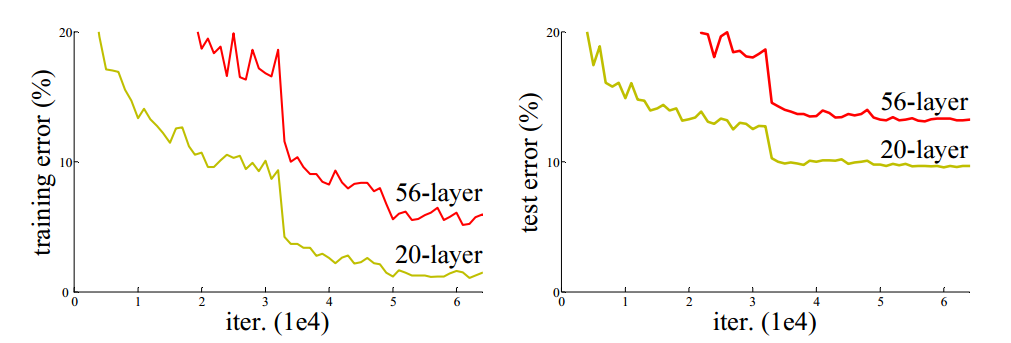
\includegraphics[width=0.8\textwidth]{figures/图片1.png}
	    \caption{层数增加无法正常训练}
	    \label{fig:1}
	\end{figure}
Deep residual learning for image recognition这篇论文就是为了解决上述“退化”问题提出的一种叫做残差网络的模型(如下图所示),该模型与之前神经网络模型不同,之前神经网络模型在输出层直接拟合期望$H(x)$,而残差神经网络并没有直接拟合期望,而是拟合$H(X) - x$这个函数,在提出这个模型的时候作者猜想,之所以加深层数之后无法对期望进行一个较好的拟合是因为求解器可能在拟合多层非线性恒等映射的问题上有困难,即假如前边层数的神经网络的已经有一个较好的输出期望,但是此时通过多层神经网络,需要将前边较好的输入与输出形成一个恒等的映射,但实验结果表明多层神经网络在形成该恒等映射上存在较大困难,因此在论文中作者提出了一种新的想法,利用残差学习重构,如果恒等映射是最优的,求解器可以简单地将多个非线性层的权值向零逼近以达到恒等映射,若非最优的,则假如多个线性层可以逐渐逼近复杂的函数,那么它也可以逐渐逼近残差函数,例如$H(X) - X$(假设输入和输出是相同维度的)。所以,我们让这些层来拟合$F(X) = H(X) - X$而不是单独的H(X)。那么原始函数就变成了$F(X) + X$。即使两种函数都可以拟合,但是,学习的难易程度是不一样的。因此该种拟合残差的方法不仅可以保证其至少不会比层数更少的神经网络差,同时每块神经网络拟合的是$F(X) = H(X) - X$而不是$H(X)$,在函数映射的复杂度上应该会更低,因此在理论层面上,该种神经网络对于解决上述“退化”问题极有可能表现出很强的优越性,论文作者在多个实验种也证明了该模型在实践层面上确实有着非常强的优越性。
	\begin{figure}[H]
	    \centering
	    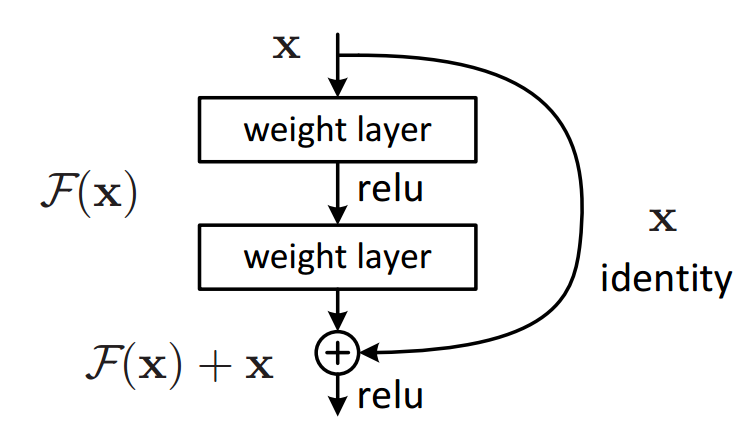
\includegraphics[width=0.5\textwidth]{figures/图片2.png}
	    \caption{残差块结构}
	    \label{fig:2}
	\end{figure}
上述残差模型解决了堆叠深度时存在的核心问题——增加深度反而导致精度下降,使得神经网络可以从十几层堆叠至几十层甚至几百层。同时该模型还有许多其他优点:
\begin{itemize}
\item 整个网络依然能够端到端地使用反向传播算法训练
\item 残差神经网络很容易地使用公共库实现,且无需修改求解器
\item 深度残差网络很容易从大幅增加的深度上获得精度提升,结果要大幅优于之前的网络。
\end{itemize}


\subsection{实现细节}

\begin{figure}[tb]
    \centering 
    \begin{tikzpicture}[
        neuron/.style={circle, draw=black, minimum size=5mm, inner sep=0},
        >=stealth,
        node distance=1.5cm
    ]
        % 定义层参数
        \def\layers{
            Input/9/0, 
            Hidden1/8/3, 
            Hidden2/6/6, 
            Output/4/9
        }
        
        % 计算最大高度(用于居中对齐)
        \pgfmathsetmacro{\maxheight}{max(9,8,6,4)*0.8}
        
        % 绘制神经元和标签
        \foreach \layername/\layercount/\x in \layers {
            % 绘制神经元(垂直居中)
            \foreach \i in {1,...,\layercount} {
                \node[neuron] (\layername-\i) at (\x, {\i*0.8 - \layercount*0.4 - 0.4}) {};
            }
            
            % 记录最下方神经元位置(第一列)
            \ifnum\x=0
                \coordinate (labelanchor) at (0, {-\layercount*0.4 - 0.6});
            \fi
            
            % 绘制标签(与第一列底部对齐)
            \node[anchor=north, align=center] at (\x, {-\layercount*0.4 - 0.6}) {\layername\\(\layercount\ 节点)};
        }
    
        % 绘制全连接线
        \foreach \i in {1,...,9}{
            \foreach \j in {1,...,8}{
                \draw[->, gray!80] (Input-\i) -- (Hidden1-\j);
            }
        }
        \foreach \i in {1,...,8}{
            \foreach \j in {1,...,6}{
                \draw[->, gray!80] (Hidden1-\i) -- (Hidden2-\j);
            }
        }
        \foreach \i in {1,...,6}{
            \foreach \j in {1,...,4}{
                \draw[->, gray!80] (Hidden2-\i) -- (Output-\j);
            }
        }
    \end{tikzpicture}	
    \caption{smallMLP网络结构}
    \label{fig:smallMLP}
\end{figure}

我们实现的一个MLP网络结构如图\ref{fig:smallMLP}所示,由于其规模较小,称为smallMLP。该网络包含一个输入层、两个隐藏层和一个输出层。输入层有9个节点,分别对应9个特征;第一个隐藏层有8个节点,第二个隐藏层有6个节点;输出层有4个节点,分别对应四类标签。每一层的神经元之间是全连接的。在这个网络中,共计使用\textbf{162}个参数。

\begin{figure}[tb]
    \centering 
    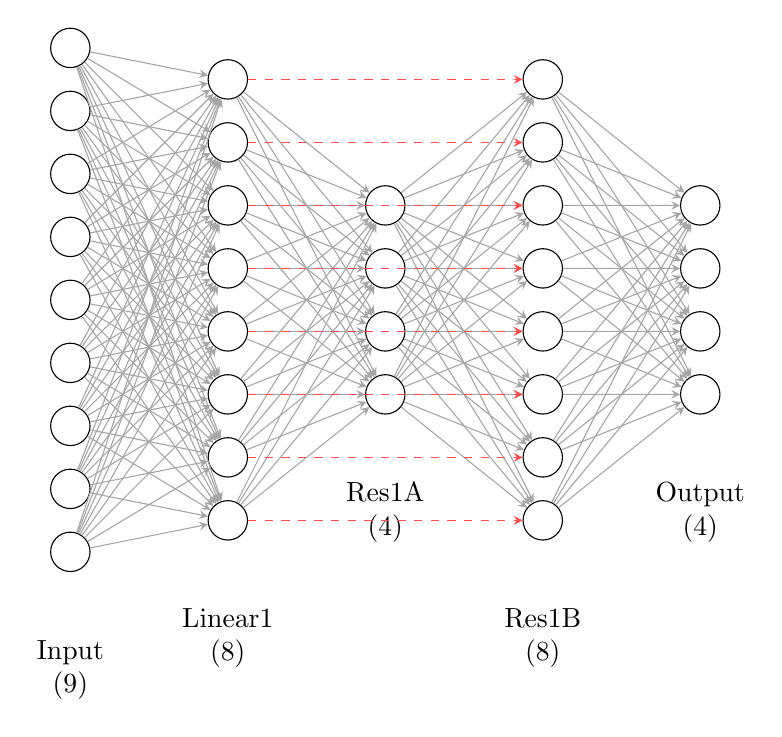
\begin{tikzpicture}[
        neuron/.style={circle, draw=black, minimum size=5mm, inner sep=0},
        >=stealth,
        node distance=1.5cm
    ]
        % 定义层参数:名称/数量/x位置
        \def\layers{
            Input/9/0, 
            Linear1/8/2, 
            Res1A/4/4, 
            Res1B/8/6,
            Output/4/8
        }

        % 绘制神经元
        \foreach \layername/\layercount/\x in \layers {
            \foreach \i in {1,...,\layercount} {
                \node[neuron] (\layername-\i) at (\x, {\i*0.8 - \layercount*0.4 - 0.4}) {};
            }
            \node[anchor=north, align=center] at (\x, {-\layercount*0.4 - 0.6}) {\layername\\(\layercount)};
        }

        % Input → Linear1
        \foreach \i in {1,...,9}{
            \foreach \j in {1,...,8}{
                \draw[->, gray!70] (Input-\i) -- (Linear1-\j);
            }
        }

        % Linear1 → Res1A
        \foreach \i in {1,...,8}{
            \foreach \j in {1,...,4}{
                \draw[->, gray!70] (Linear1-\i) -- (Res1A-\j);
            }
        }

        % Res1A → Res1B
        \foreach \i in {1,...,4}{
            \foreach \j in {1,...,8}{
                \draw[->, gray!70] (Res1A-\i) -- (Res1B-\j);
            }
        }

        % 残差连接(Linear1 → Res1B):虚线
        \foreach \i in {1,...,8}{
            \draw[->, dashed, red!70] (Linear1-\i) -- (Res1B-\i);
        }

        % Res1B → Output
        \foreach \i in {1,...,8}{
            \foreach \j in {1,...,4}{
                \draw[->, gray!70] (Res1B-\i) -- (Output-\j);
            }
        }

    \end{tikzpicture}	
    \caption{SmallResNet 网络结构(含残差连接)}
    \label{fig:SmallResNet}
\end{figure}


另一方面,我们还实现了一个小型的残差网络(smallResNet)如图\ref{fig:SmallResNet}所示,以期能取得更好的效果。该网络大体结构与smallMLP相同,但对于残差连接结构,使用了$8\rightarrow4\rightarrow8$的结构。Linear1层的输出结果,会直接与Res1A层的输出结果相加,作为Res1B层的输入,即图\ref{fig:SmallResNet}中的红色虚线所示。在这个网络中,共计使用\textbf{192}个参数。

\subsection{性能评估}

使用多层感知机与残差网络对数据集进行训练,得到如表\ref{tab:Classic Model Training Results}所示的实验结果。

\begin{table}[H]
\centering
\caption{经典模型的训练结果}
\label{tab:Classic Model Training Results}
\begin{tabular}{ccccc}
    \toprule
    \textbf{迭代次数} & \textbf{经典模型} & \textbf{训练准确率} & \textbf{测试准确率} & \textbf{测试F1分数} \\
    \midrule
    \multirow{2}{*}{50} & SmallMLP & 69.55\% & 66.10\% & 0.3993 \\
        & SmallResNet & 74.37\% & 75.30\% & 0.5564 \\
    \midrule
    \multirow{2}{*}{250} & SmallMLP & 86.98\% & 85.60\% & 0.6645 \\
        & SmallResNet & 87.02\% & 85.50\% & 0.6632 \\
    \midrule
    \multirow{2}{*}{500} & SmallMLP & 87.15\% & 85.50\% & 0.6635 \\
        & SmallResNet & 87.37\% & 85.80\% & 0.6662 \\
    \bottomrule
\end{tabular}
\end{table}

根据实验结果可知,在固定参数大小下,经典的神经网络模型ResNet与MLP的实验精度基本一样,使用更复杂的ResNet模型对实验的结果精度并未产生较大提升。从模型理论上看,由于更复杂的模型(ResNet)在提出的时候往往是解决增加模型参数却不能极大提高准确率的问题,而在该任务中所用经典参数较少,并未达到MLP的模型性能极限,因此使用ResNet并未提升较大精度。

由以上实验分析,我们可以提出如下假设:在固定参数下,存在经典模型并未超出其性能极限,即在固定参数下更改模型并不能提升预测精度。在此假设下,我们希望存在某种模型能够在原有经典模型的基础上,能进一步较大提升模型的预测精度,从而减少模型的参数量,进而提高模型的计算效率。

%%%%%%%%%%%%%%%%%%%%%%%%%%%%%%%%%%%%%%%%%%%%%%%%%%%%%%%%%%%%%%%%%%%%%%%%%%%%%%%%%%%%%%%%%%%%%%%%%%%%%%%%%%%%%%%%%%%%%%%%%%%%%%%

\section{量子机器学习模型}

\subsection{算法原理}

\begin{algorithm}[H]
    \caption{QMLP训练流程}
    \label{alg:qmlp_train}
    \begin{algorithmic}[1]
    \State 初始化参数$\{\theta_l\}_{l=1}^L$和$\{f_l\}_{l=1}^L$
    \For{每个训练epoch}
        \State 编码输入:$\ket{\phi_0} = S(\mathbf{x})\ket{0}^{\otimes N}$
        \State 量子态演化:$\ket{\phi_L} = \prod_{l=1}^L U_l(\theta_l)\ket{\phi_0}$
        \State 参数化纠缠: $\ket{\phi_L} = \bigotimes_{m=1}^{N/2} CRX(\phi_m)\ket{\phi_L}$
        \State 重传:$\ket{\phi_L} = R_l(\mathbf{x})\ket{\phi_L}$
        \State 测量期望值:$\langle Z\rangle_i = \bra{\phi_L} Z_i \ket{\phi_L}$
        \State 计算损失:$\mathcal{L} = -\sum_c y_c \log p_c$
        \State 通过参数偏移规则更新参数
    \EndFor
    \end{algorithmic}
\end{algorithm}

\begin{figure}[htbp]
    \centering
    \smartdiagram[flow diagram:horizontal]{
        输入$\mathbf{x}$,
        线性编码,
        变分层1,
        参数化纠缠,
        RUU重传,
        变分层2,
        输出测量和优化
    }
    \caption{QMLP算法流程图}
    \label{fig:qmlp_flow_smart}
\end{figure}
在本次报告中,我们实现的量子机器学习模型为QMLP(Quantum Multi-Layer Perceptron)\cite{chu2022qmlperrortolerantnonlinearquantum},流程如算法\ref{alg:qmlp_train}和图\ref{fig:qmlp_flow_smart}所示。

QMLP是基于变分量子算法的量子神经网络模型,主要由以下几个部分组成:
\subsubsection{量子数据编码}

QMLP采用线性旋转编码将经典数据映射到量子态:

\begin{equation}
S(\mathbf{x}) = \bigotimes_{k=1}^N RX(x_k)
    \label{eq:linear_encoding}
\end{equation}
这个电路都构造非常简单,如图\ref{fig:Quantum Circuits}左图所示。由此我们将经典数据映射到量子态,同时通过单比特旋转门独立编码每个输入特征,达到抑制噪声传播的目的。

\begin{figure}[tb]
\centering
    \begin{quantikz}
        \lstick{$\ket{0}$} & \gate{RX(x_1)} & \\
        \lstick{$\ket{0}$} & \gate{RX(x_2)} & \\
        \lstick{$\vdots$} \wave&&& \\
        \lstick{$\ket{0}$} & \gate{RX(x_N)} &
    \end{quantikz}
    \qquad
    \begin{quantikz}
        \lstick{$\ket{\psi_1}$} & \ctrl{1} & \gate{RX(\theta_1)} & \\
        \lstick{$\ket{\psi_2}$} & \targ{}{} & \gate{RY(\theta_2)} &
    \end{quantikz}
\caption{左:量子数据编码电路;右:参数化纠缠层电路}
\label{fig:Quantum Circuits}
\end{figure}

\subsubsection{变分量子电路}
在对输入进行量子编码后,便可以对其应用式\ref{eq:variational_circuit}对应的变分量子电路进行参数化幺正变换(类似于经典神经网络中的权重矩阵乘法)。
\begin{equation}
    \ket{\phi_L} = \prod_{l=1}^L U_l(\theta_l)\ket{\phi_0}
    \label{eq:variational_circuit}
\end{equation}
$U_l(\theta_l)$表示由一组可训练参数$\theta_l$控制的幺正变换,$\ket{\phi_0}$表示编码后的输入态。\\
然后相邻量子比特之间应用CRX门(式\ref{eq:entanglement})创建纠缠,增强局部关联性。电路如图\ref{fig:Quantum Circuits}右图所示。
\begin{equation}
    \ket{\phi_L} = \bigotimes_{m=1}^{N/2} CRX(\phi_m)\ket{\phi_L}
    \label{eq:entanglement}
\end{equation}
CRX门的矩阵表达为式\ref{eq:crx}。
\begin{equation}
    CRX(\theta) = \begin{pmatrix}
    1 & 0 & 0 & 0 \\
    0 & 1 & 0 & 0 \\
    0 & 0 & \cos\theta/2 & -i\sin\theta/2 \\
    0 & 0 & -i\sin\theta/2 & \cos\theta/2 
    \label{eq:crx}
    \end{pmatrix}
\end{equation}
\subsubsection{重上传单元}
接着对每一位输入进行重传(式\ref{eq:ruu}),重复注入编码层$S(\mathbf{x})$在变分电路中生成输入的高阶项引入非线性(类似于经典电路的激活函数),增强量子神经网络的表达能力。
\begin{equation}
    \ket{\phi_L} = R_l(\mathbf{x})\ket{\phi_L}
    \label{eq:ruu}
\end{equation}
$R_l$表示所用的重传单元如$RX$,$RY$门
\subsubsection{测量与优化}
通过Pauli-Z基测量(式\ref{eq:measurement})将处理后的量子态转换为经典可读信号,然后便可应用经典方法如Adam优化算法等对模型参数进行优化。
\begin{equation}
    \langle Z_i \rangle = \bra{\phi_L} Z_i \ket{\phi_L} \in [-1, 1]
    \label{eq:measurement}
\end{equation}


\subsection{实现细节}

出于效率的考量,我们采用了量子经典混合的架构,即首先由经典神经网络将9维的输入降维到4维,之后将这些数据输入到QMLP中,最后的测量结果就是输出。整个架构如图\ref{fig:QuantumMLP}之子图1所示,而其中的"Quantum Circuit"部分具体如图\ref{fig:QuantumMLP}之子图2所示。在子图2中,$Rot(\theta_{i}\sim\theta_{i+2})$表示了一套需要三个量子参数的$RX,RY,RZ$门组合;而四个相连受控位表示一套$CRX$门组合,需要四个量子参数,分别如图\ref{fig:QuantumMLP}之子图3,4所示。显而易见,在这个架构中,经典参数量为$9\times4+4=40$,而量子参数量为$8\times3+2\times4=32$个,总共\textbf{72}个参数。

\begin{figure}[htb]
\centering
    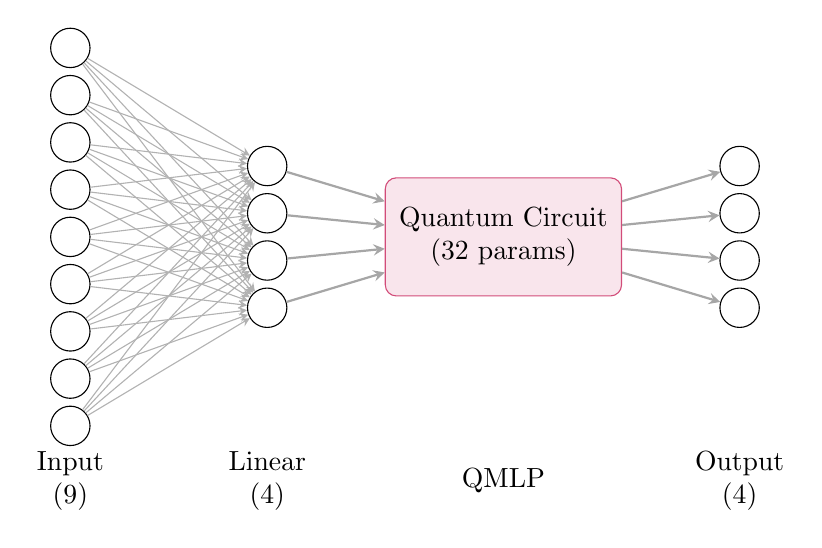
\begin{tikzpicture}[
        neuron/.style={circle, draw=black, minimum size=5mm, inner sep=0},
        quantum/.style={rectangle, draw=purple!70, fill=purple!10, minimum width=3cm, minimum height=1.5cm, rounded corners, align=center},
        >=stealth,
        every label/.style={text width=2cm, align=center}
    ]

        % 定义各层节点数及间距
        \def\inputN{9}
        \def\linearN{4}
        \def\outputN{4}
        \def\dy{0.6}  % 垂直间距

        % 计算最大层数以居中对齐
        \pgfmathsetmacro{\maxN}{max(\inputN,\linearN,\outputN)}
        \pgfmathsetmacro{\centerY}{(\maxN - 1) * \dy / 2}

        % Input layer
        \foreach \i in {1,...,\inputN} {
            \pgfmathsetmacro{\y}{(\i - 1) * \dy - (\inputN - 1) * \dy / 2}
            \node[neuron] (input-\i) at (0, \y) {};
        }
        \node[align=center] at (0, -\centerY - 0.7) {Input\\(\inputN)};

        % Linear layer
        \foreach \i in {1,...,\linearN} {
            \pgfmathsetmacro{\y}{(\i - 1) * \dy - (\linearN - 1) * \dy / 2}
            \node[neuron] (linear-\i) at (2.5, \y) {};
        }
        \node[align=center] at (2.5, -\centerY - 0.7) {Linear\\(\linearN)};

        % Quantum Circuit block(居中即可)
        \node[quantum] (quantum) at (5.5, 0) {Quantum Circuit\\(32 params)};
        \node at (5.5, -\centerY - 0.7) {QMLP};

        % Output layer
        \foreach \i in {1,...,\outputN} {
            \pgfmathsetmacro{\y}{(\i - 1) * \dy - (\outputN - 1) * \dy / 2}
            \node[neuron] (output-\i) at (8.5, \y) {};
        }
        \node[align=center] at (8.5, -\centerY - 0.7) {Output\\(\outputN)};

        % Input → Linear
        \foreach \i in {1,...,\inputN}{
            \foreach \j in {1,...,\linearN}{
                \draw[->, gray!60] (input-\i) -- (linear-\j);
            }
        }

        % Linear → Quantum
        \foreach \i in {1,...,\linearN}{
            \draw[->, thick, gray!70] (linear-\i) -- (quantum);
        }

        % Quantum → Output
        \foreach \i in {1,...,\outputN}{
            \draw[->, thick, gray!70] (quantum) -- (output-\i);
        }

    \end{tikzpicture} \\

    % \vspace{0.1cm}
    \noindent\makebox[\textwidth]{\dotfill}
    \vspace{0.01cm}

    \begin{quantikz}[row sep=0.3cm, column sep=0.5cm]
        \lstick{$q_0$} & \gate{R_x(x_0)} & \gate{Rot(\theta_0\sim\theta_2)} & \ctrl[vertical wire=c]{3} & \gate{R_x(x_0)} & \gate{Rot(\theta_{16}\sim\theta_{18})} & \ctrl[vertical wire=c]{3} & \meter{} \\
        \lstick{$q_1$} & \gate{R_x(x_1)} & \gate{Rot(\theta_3\sim\theta_5)} & \control{}   & \gate{R_x(x_1)} & \gate{Rot(\theta_{19}\sim\theta_{21})} & \control{}   & \meter{} \\
        \lstick{$q_2$} & \gate{R_x(x_2)} & \gate{Rot(\theta_6\sim\theta_8)} & \control{} & \gate{R_x(x_2)} & \gate{Rot(\theta_{22}\sim\theta_{24})} & \control{} & \meter{} \\
        \lstick{$q_3$} & \gate{R_x(x_3)} & \gate{Rot(\theta_9\sim\theta_{11})} & \control{}   & \gate{R_x(x_3)} & \gate{Rot(\theta_{25}\sim\theta_{27})} & \control{}   & \meter{} \\
    \end{quantikz} \\

    \noindent\makebox[\textwidth]{\dotfill}
    \vspace{0.01cm}

    \begin{quantikz}
        & \gate{Rot((\theta_{i}\sim\theta_{i+2}))} & 
    \end{quantikz} \quad=\quad \begin{quantikz}[column sep=0.1cm]
        & \gate{RX(\theta_{i})} & \gate{RY(\theta_{i+1})} & \gate{RZ(\theta_{i+2})} & 
    \end{quantikz} \\

    \noindent\makebox[\textwidth]{\dotfill}
    \vspace{0.01cm}

    \begin{quantikz}
        & \ctrl[vertical wire=c]{3} & \\ & \control{} & \\ & \control{} & \\ & \control{} &
    \end{quantikz} \quad=\quad \begin{quantikz}[row sep=0.04cm, column sep=0.05cm]
        & \ctrl{1} & & & \gate{RX(\theta_{i+3})} &\\
        & \gate{RX(\theta_{i})} & \ctrl{1} & & & \\
        & & \gate{RX(\theta_{i+1})} & \ctrl{1} & & \\
        & & & \gate{RX(\theta_{i+2})} & \ctrl{-3} &
    \end{quantikz}

\caption{\centering 自上而下:子图1:QuantumMLP 网络结构图:线性映射 + 参数化量子电路 + 测量输出;\\ 子图2:参数化量子电路的具体实现;\\ 子图3:$Rot(\theta_{i}\sim\theta_{i+2})$门的具体实现;\\ 子图4:$CRX$门组合的具体实现。}
\label{fig:QuantumMLP}
\end{figure}

% \begin{quantikz}[row sep=0.5cm, column sep=0.5cm]
%     \lstick{$q_0$} & \gate{R_x(x_0)} & \gate{Rot(\theta_0)} & \ctrl{1} & \gate{R_x(x_0)} & \gate{Rot(\theta_1)} & \ctrl{1} & \meter{} \\
%     \lstick{$q_1$} & \gate{R_x(x_1)} & \gate{Rot(\theta_3)} & \targ{} & \gate{R_x(x_1)} & \gate{Rot(\theta_4)} & \targ{} & \meter{} \\
%     \lstick{$q_2$} & \gate{R_x(x_2)} & \gate{Rot(\theta_6)} & \ctrl{1} & \gate{R_x(x_2)} & \gate{Rot(\theta_7)} & \ctrl{1} & \meter{} \\
%     \lstick{$q_3$} & \gate{R_x(x_3)} & \gate{Rot(\theta_9)} & \targ{} & \gate{R_x(x_3)} & \gate{Rot(\theta_{10})} & \targ{} & \meter{}
% \end{quantikz}


\subsection{性能评估}

使用如图\ref{fig:QuantumMLP}的结构对数据集进行训练,得到如表\ref{tab:Quantum Classic Model Training Results}所示的实验结果。

\begin{table}[H]
    \centering
    \caption{量子经典混合模型的训练结果}
    \label{tab:Quantum Classic Model Training Results}
    \begin{tabular}{cccc}
        \toprule
        \textbf{迭代次数} & \textbf{训练准确率} & \textbf{测试准确率} & \textbf{测试F1分数} \\
        \midrule
        50 & 75.98\% & 76.60\% & 0.6004 \\
        250 & 92.95\% & 90.80\% & 0.8880 \\
        500 & 93.33\% & 90.90\% & 0.8820 \\
        \bottomrule
    \end{tabular}
\end{table}

对比表\ref{tab:Classic Model Training Results},我们可以显著发现量子经典混合模型有着更高的收敛速度,收敛之后的准确率与F1分数也更高。

%%%%%%%%%%%%%%%%%%%%%%%%%%%%%%%%%%%%%%%%%%%%%%%%%%%%%%%%%%%%%%%%%%%%%%%%%%%%%%%%%%%%%%%%%%%%%%%%%%%%%%%%%%%%%%%%%%%%%%%%%%%%%%%

\section{性能对比与分析}

\subsection{性能对比}

\begin{table}[H]
    \centering
    \caption{经典机器学习与量子机器学习的性能对比}
    \label{tab:Performance Comparison of Classical and Quantum Models}
    \begin{tabular}{ccccc}
        \toprule
        \textbf{模型} & \textbf{参数量} & \textbf{训练准确率} & \textbf{测试准确率} & \textbf{测试F1分数} \\
        \midrule
        经典小型ResNet & 192 & 87.37\% & 85.80\% & 0.6662 \\
        量子经典混合MLP & 72 & 93.33\% & 91.00\% & 0.8820 \\
        \bottomrule
    \end{tabular}
\end{table}

通过上表我们得知,混合了经典MLP与量子MLP的模型,在使用参数量远远小于经典小型ResNet的情况下,取得了更好的训练准确率、测试准确率和F1分数。我们可以认为,量子MLP在该数据集上取得了比经典MLP更好的性能。

\subsection{差异分析}
\begin{table}[H]
    \centering
    \caption{量子与经典神经网络核心组件对比}
    \label{tab:quantum_classical}
    \begin{tabular}{ccccc}
        \toprule
        \textbf{功能} & \textbf{经典神经网络组件} & \textbf{QMLP组件} \\
        \midrule
        输入编码 & 数据标准化层 & 单比特旋转门编码 \\
        & $\mathbf{x} \in \mathbb{R}^n \to \text{Norm}(\mathbf{x})$ & $S(\mathbf{x}) = \bigotimes_k RX(x_k)$ \\
        \midrule
        特征变换 & 全连接层 & 变分量子电路 \\
        & $W\mathbf{x} + \mathbf{b}$ & $U(\theta)\ket{\phi}$ \\
        \midrule
        非线性引入 & 激活函数 & 数据重上传单元(RUU) \\
        & $\text{ReLU}(x)=\max(0,x)$ & $R_l(\mathbf{x}) = RX(f_l(\mathbf{x}))$ \\
        \midrule
        参数优化 & 梯度下降 & 参数偏移规则 \\
        & $\theta \leftarrow \theta - \eta \nabla_\theta \mathcal{L}$ & $\nabla_\theta \langle Z\rangle \approx \frac{\langle Z\rangle_{\theta+\delta} - \langle Z\rangle_{\theta-\delta}}{2}$ \\
        \midrule
        输出处理 & Softmax分类层 & Pauli-Z测量 \\
        & $p_c = \frac{e^{y_c}}{\sum e^{y_i}}$ & $\langle Z\rangle_i = \bra{\psi}Z_i\ket{\psi}$ \\
        \bottomrule
    \end{tabular}
\end{table}
%%%%%%%%%%%%%%%%%%%%%%%%%%%%%%%%%%%%%%%%%%%%%%%%%%%%%%%%%%%%%%%%%%%%%%%%%%%%%%%%%%%%%%%%%%%%%%%%%%%%%%%%%%%%%%%%%%%%%%%%%%%%%%%

\section{总结}

%插入表格(三线表)
% \begin{table}[htbp]
%     \centering
%     \caption{表题}
%     \begin{tabular}{ccccc}%{{5}{c}}

%         \toprule
%         {组别} & {物理量1/单位} & {物理量2/单位} & {物理量3/单位} & {物理量4/单位} \\
%         \midrule
%         A&{}&{}&{}&{}\\
%         B&{}&{}&{}&{}\\
%         C&{}&{}&{}&{}\\
%         D&{}&{}&{}&{}\\
%         \bottomrule
%     \end{tabular}
% \end{table}


%插入图片
% \begin{figure}[htbp]
%     \centering 
%     \includegraphics[height=5.99cm,width=8.25cm]{E:/engineer file/latex/learn1/photo/test.png}
%     \caption{图注}
% \end{figure}
%table和figure为浮动体






%%%%%列出参考文献%%%%%
\vspace{12pt}
\zihao{-5}%设置参考文献字号
\bibliography{references.bib}%调用bib文件 加入参考文献
%知网复制出的latex代码比工大图书馆复制出的latex代码好用

%%%%%%%%%%%%%%%附录部分%%%%%%%%%%%%%%%
% \newpage
% \appendix%设置附录
% \zihao{-5}%设置附录字号
% \section*{附录一:}




\end{document}